\chapter{Аналитический раздел}
\vspace{-0.5cm}\hspace{0.6cm}В данном разделе производится анализ и сравнение методов и алгоритмов предметной области, необходимых для выполнения поставленной задачи.

\section{Постановка технического задания}
\hspace{0.6cm}Необходимо разработать программу моделирования анимации развевающегося на ветру флага на флагштоке методом ключевых кадров. Для каждого промежуточного кадра программа должна рассчитывать текущее положение точек поверхности флага. Должен быть задан набор законов управления движением при переходе между двумя соседними ключевыми кадрами. Исследовать возможность учёта освещённости, оптических свойств поверхностей. Источником света является солнце.

\vspace{0.3cm}В данной задаче можно выделить следующие подзадачи:

\begin{itemize}
	\item реализация процедуры создания объектов сцены;
	\item анализ, выбор и реализация алгоритма удаления невидимых линий;
	\item анализ, выбор и реализация алгоритма закраски объекта;
	\item реализация камеры и источника света;
	\item реализация анимации при помощи метода ключевых кадров на основе законов движения;
	\item реализация пользовательского интерфейса.
\end{itemize}

\section{Формализация объектов синтезируемой сцены}
\hspace{0.6cm}Сцена включает в себя следующие объекты: флагшток, закреплённый на нём флаг, платформа, на котором стоит флагшток с флагом.

\vspace{0.3cm}Флагшток представляет из себя тонкий длинный цилиндр с наконечником в виде полусферы. Определяется координатами центра нижнего основания, диаметром оснований и высотой. Радиус полусферы наконечника флагштока равен диаметру основания флагштока.

\vspace{0.3cm}Флаг представляет из себя прямоугольное полотнище с отношением ширины к длине 2:3. Ширина флага равна 1/6 части высоты флагштока. Определяется координатами точки крепления верхней части флага, шириной и длиной. Для придания гибкости флагу полотнище разбивается на несколько треугольников. 

\vspace{0.3cm}Платформа определяется прямоугольным параллелепипедом с квадратным основанием. В центре имеется отверстие в форме цилиндра, радиус которого равен радиусу цилиндра. Таким образом центр основания флагштока совпадает с центром нижней грани платформы.

\section{Законы управления движением точек объектов}
\hspace{0.6cm}Для решения задачи расчёта нового положения точек поверхности флага следует определить вектор скорости точки в определённый момент времени. Для этого необходимо проанализировать физические факторы, определяющие движение точки.

\vspace{0.3cm}Если распределить массу флага $M$ по всем точкам его поверхности, то можно говорить о силах, действующих на точку поверхности. Чтобы сдвинуть точки, в которых флаг крепится к флагштоку, необходимо приложить бесконечно большую силу. Будем считать, что точки, в которых флаг крепится к флагштоку, невесомыми, чтобы не учитывать воздействие сил на данные точки (их масса $m = 0$). Рассмотрим силы, воздействующие на остальные точки флага.

\vspace{0.3cm}Так как точка имеет массу, то на неё воздействует сила гравитации $\vec{F}_{grav}$, направленная к земле. Вектор этой силы определён одинаковым образом для каждой точки:

\begin{equation}
\vec{F}_{grav} = m\vec{g} ,
\end{equation}
где $m$ - масса точки, $\vec{g}$ - вектор ускорения свободного падения.

\vspace{0.3cm}Точки поверхности между собой связаны, потому на каждую из них действуют силы упругости ткани $\vec{F}_{spring}$. Силы упругости стремятся вернуть точки в исходное состояние. Так как точки поверхности связаны между собой рёбрами, то эти рёбра могут выступать в качестве пружин. Каждая такая пружина имеет свою жёсткость и длину в состоянии покоя. Вектор силы воздействия пружины на точки рассчитывается по закону Гука
\begin{equation}
\vec{F}_{spring} = k\vec{x} ,
\end{equation}
где $k$ - коэффициент жёсткости пружины, $\vec{x}$ - вектор изменения длины пружины, направленный вдоль пружины.

\vspace{0.3cm}Направление силы определяется вектором $\vec{x}$, то есть тем, растянута или сжата пружина: если $\vec{x}$ направлен от точки, то пружина растянута, если к точке - сжата.

\vspace{0.3cm}Сила ветра прикладывается ко всем граням ткани флага, поэтому необходимо вначале определить вектор направления силы, создаваемой ветром в каждой точке. Для этого находим сначала векторы нормали $\vec{n}$ к каждой грани, после чего нормаль умножаем на проекцию вектора ветра $\vec{w}$ к вектору нормали, тем самым получая вектор силы воздействия ветра на грань.

\begin{center}
	$\vec{F}_{w} = \vec{n} \cdot pr_{\vec{n}}\vec{w} =$
	$\vec{n} \cdot \displaystyle \frac{\vec{n} \cdot \vec{w}}{|\vec{n}|} =$
	$\vec{n} \cdot (\vec{n} \cdot \vec{w})$\\
\end{center}

Таким образом, получаем, что силы воздействия ветра на грань
\begin{equation}
\displaystyle \vec{F}_{wi} = \vec{n} \cdot (\vec{n} \cdot \vec{w}),
\end{equation}
где $\vec{n} \cdot \vec{w}$ - скалярное произведение, $i$ - номер грани.

\vspace{0.3cm}Так как каждая точка являются частью одновременно нескольких граней (кроме угловых точек, каждая из них принадлежит одной грани), то результирующий вектор силы воздействия ветра $\vec{F}_{wind}$ для данной точки равен сумме векторов воздействия на грани.
\begin{equation}
\displaystyle \vec{F}_{wind} = \sum_{i=1}^n \vec{F}_{wi},
\end{equation}
где $\vec{F}_{wi}$ - сила воздействия ветра на i-ую грань, $i$ - номер грани, которой принадлежит вершина, $n$ - число граней, в которые входит данная вершина.

\vspace{0.3cm}Замедляется движение точек поверхности под воздействием сил трения. Без трения движение может никогда не прекратиться. Вектор силы трения $\vec{F}_{fric}$ определяется следующим образом:

\begin{equation}
\vec{F}_{fric} = -\mu\vec{F},
\label{eq:fric}
\end{equation}
где $\mu$ - коэффициент трения, $\vec{F}$ - результирующая сила, действующая на точку.

Как видно из уравнения \ref{eq:fric}, сила трения направлена в обратную от результирующей силы сторону, чем и замедляет движение.

\vspace{0.3cm}После определения всех составляющих сил определяется вектор результирующей силы $\vec{F}$ как сумма составных

\begin{equation}
\vec{F} = \vec{F}_{grav} + \vec{F}_{spring} + \vec{F}_{fric} + \vec{F}_{wind}.
\end{equation}

По второму закону Ньютона определяется ускорение точки

\begin{equation}
\displaystyle \vec{a} = \frac{\vec{F}}{m}.
\label{eq:accel}
\end{equation}

\vspace{0.3cm}Для того чтобы сократить число вычислений и чтобы не считать каждую миллисекунду новое значение ускорения $\vec{a}$, воспользуемся интегрированием для вычисления ускорения $\vec{a}$, достигнутого за заданный промежуток времени $t$
\begin{equation}
\displaystyle \vec{a} = t\frac{\vec{F}}{m}.
\end{equation}
По найденному ускорению определяется новая скорость движения точки $\vec{v}$
\begin{equation}
\vec{v} = \vec{v}_{0} + \vec{a}t,
\end{equation}
где $\vec{v}_{0}$ - предыдущее значение скорости.
Исходя из полученного вектора скорости определяются новые координаты $(x, y, z)$ заданной точки:
\begin{equation}
(x, y, z) = (x_{0} + v_{x}, y_{0} + v_{y}, z_{0} + v_{z}) ,
\end{equation}
где $(x_{0}, y_{0}, z_{0})$ - координаты предыдущего положения точки,
$(v_{x}, v_{y}, v_{z})$ - координаты вектора скорости $\vec{v}$.

\vspace{0.3cm}Таким образом, итоговая система уравнений, определяющая движение незакреплённых точек поверхности полотна флага, имеет следующий вид:

\begin{equation}
\begin{cases}
\vec{F}_{grav} = m\vec{g}\\
\vec{F}_{spring} = k\vec{x}\\
\vec{F}_{fric} = -\mu\vec{F}\\
\vec{F}_{wi} = \vec{n} \cdot (\vec{n} \cdot \vec{w})\\
\vec{F}_{wind} = \sum\limits_{i=1}^n \vec{F}_{wi}\\
\vec{F} = \vec{F}_{grav} + \vec{F}_{spring} + \vec{F}_{fric} + \vec{F}_{wind}\\
\displaystyle \vec{a} = t\frac{\vec{F}}{m}\\
\vec{v} = \vec{v}_{0} + \vec{a}t\\
(x, y, z) = (x_{0} + v_{x}, y_{0} + v_{y}, z_{0} + v_{z})\\
\end{cases}.
\label{eq:sys}
\end{equation}

\section{Визуализация}

\subsection{Алгоритм Брезенхема}
\hspace{0.6cm}Алгоритм Брезенхема построения отрезков выбирает оптимальные растровые координаты для представления отрезка, другими словами, данный алгоритм позволяет получить приближение идеальной прямой точками растровой сетки.

\vspace{0.3cm}Основная идея алгоритма базируется на расстоянии между действительным положением отрезка и ближайшими координатами сетки. Это расстояние называют ошибкой\cite{book:rojers}.

\vspace{0.3cm}В данном алгоритме проверяется принадлежность проекции к оси x или y. На какую ось проекция будет больше, на ту ось и смещается пиксель. По другой оси смещение на один пиксель проискходить лишь в том случае, когда линия отклонилось от оси более чем на половину пикселя.

\vspace{0.3cm}Преимущество:
\begin{itemize}
	\item высокая скорость растрирования вектора.
\end{itemize}

\vspace{0.3cm}Недостатки:
\begin{itemize}
	\item при маленьком разрещении экрана наблюдается эффект ступенчатости;
	\item округление значений: действительные величины преобразуются в ближайшие целые числа. 
\end{itemize}

\subsection{Удаление невидимых линий}
\hspace{0.6cm}Удаление невидимых линий и поверхностей не самая простая задача в компьютерной графике: на данный момент не существует такого алгоритма, который работал бы быстро и с высокой детализацией результата. Под детализацией понимается: просчет теней, прозрачности, фактуры, отражения и преломления света.

\vspace{0.3cm}Алгоритмы удаления невидимых линий и поверхностей делятся на два вида:
\begin{itemize}
	\item алгоритмы, работающие в пространстве изображения;
	\item алгоритмы, работающие в объектном пространстве.
\end{itemize}

\vspace{0.3cm}В алгоритмах первого вида находятся ближайшие точки сцены к наблюдателю и отображаются. Такой подход к удалению невидимых линий и поверхностей не требует высокой точности вычислений, поэтому сложности таких алгоритмов не превышает $O(c \cdot n)$, где $c$ - число пикселей, $n$ - число объектов \cite{machinegraph}. В алгоритмах данного вида точность ограничивается разрешающей способностью экрана.

\vspace{0.3cm}В алгоритмах второго вида все действия происходят в физической системе координат, в которой описаны данные объекты. Сложность таких алгоритмов в среднем для n объектов $O(n^2)$\cite{machinegraph}. Однако, медленная скорость работы обусловлена точными результатами. Качество, полученных изображений, не будет зависеть от разрешений экрана.

\vspace{0.3cm}В рамках курсового проекта необходимо выбрать такой алгоритм, который бы быстро удалял задние линии и поверхности, поэтому выбор осуществлялся между следующими алгоритмами:
\begin{itemize}
	\item алгоритм художника;
	\item алгоритм Z-буфера;
	\item алгоритм A-буфера.
\end{itemize}
\vspace{0.3cm}Рассмотрим каждый из данных алгоритмов, сравним достоинства и недостатки и определим, какой из алгоритмов лучше подходит для решения нашей задачи.

\subsubsection{Алгоритм художника}
\hspace{0.6cm}Алгоритм художника является простейшим вариантом решения задачи об удалении невидимых линий и граней в компьютерной графике.

\vspace{0.3cm}Название <<алгоритм художника>> был использован в связи с тем, что его реализация схожа с техникой, которой пользуются многие живописцы: сначала рисуют дальние части сцены, затем ближние части. Так и в алгоритме художника: многоугольники сортируются по координате z по возрастанию, в начале расположены те грани, которые расположены ближе всего к наблюдателю. После того, как грани отсортированы по расстоянию от наблюдателя, их начинают отрисовывать на сцене, начиная с самых дальних.

\vspace{0.3cm}Главным недостатком данного алгоритма является неправильное вычислений задних граней при определенных сценариях: когда один многоугольник является относительно одной фигуры неэкранируемым, а относительно другой является экранируемым. Данную проблему можно наблюдать на рис. \ref{fig:painter}.

\vspace{0.3cm}Также этот алгоритм работает медленно, из-за отрисовки ненужных задних граней, которые по итогу будут закрашены ближней гранью к наблюдателю. Также если задних граней будет много, то данный алгоритм будет весьма трудозатратным.

\begin{figure}[ht!]
	\centering
	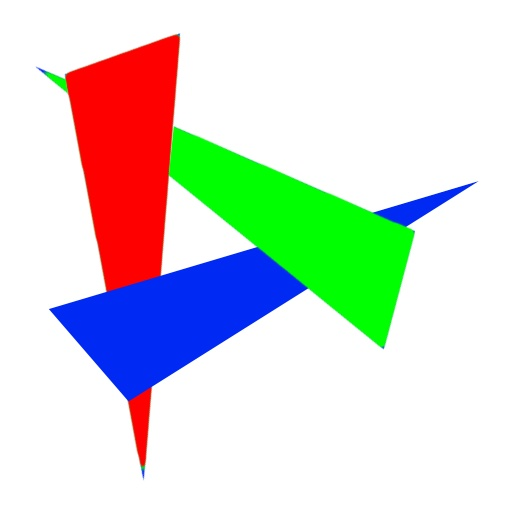
\includegraphics[scale=0.6]{painter}
	\caption{Ошибочный вариант расположения фигур для алгоритма художника}
	\label{fig:painter}
\end{figure}

\newpage

\subsubsection{Алгоритм Z-буфера}
\hspace{0.6cm}Алгоритм Z-буфера заключается в том, что помимо буфера кадра (матрицы, в которой содержится информация о цвете для каждого пикселя в пространстве изображения) используется также так называемый Z-буфер, в котором хранится координата z для каждого пикселя, т. е. его глубина.

\vspace{0.3cm}Во время работы алгоритма, значение Z-буфера или глубины сравнивается со значением, который нужно занести в Z-буфер. Если сравнение показывает, что новое значение расположено ближе к наблюдателю по оси $z$, то новый пиксель заносится в буфер кадра, а в Z-буфер заносится новое значение глубины. Можно сказать, что алгоритм выполняет поиск наибольшего значения функции $z(x,y)$ по $x$ и $y$. Визуализацию работы алгоритма можно посмотреть на рис. \ref{fig:zbuffer}.

\vspace{0.3cm}Данный алгоритм является быстродейственным, так как в нем не выполняются лишние операции, в отличие от алгоритма художника.

\vspace{0.3cm}Существенными недостатками являются:
\begin{itemize}
	\item для хранения буферов требуется большой объём памяти\cite{kurov};
	\item пиксели в буфер кадра заносятся в произвольном порядке, поэтому появляются трудности с реализацией эффектов прозрачности или просвечивания.
\end{itemize}

Вторую проблему можно решить, если заранее известно, из каких материалов состоит объект.

\begin{figure}[ht!]\
	\centering
	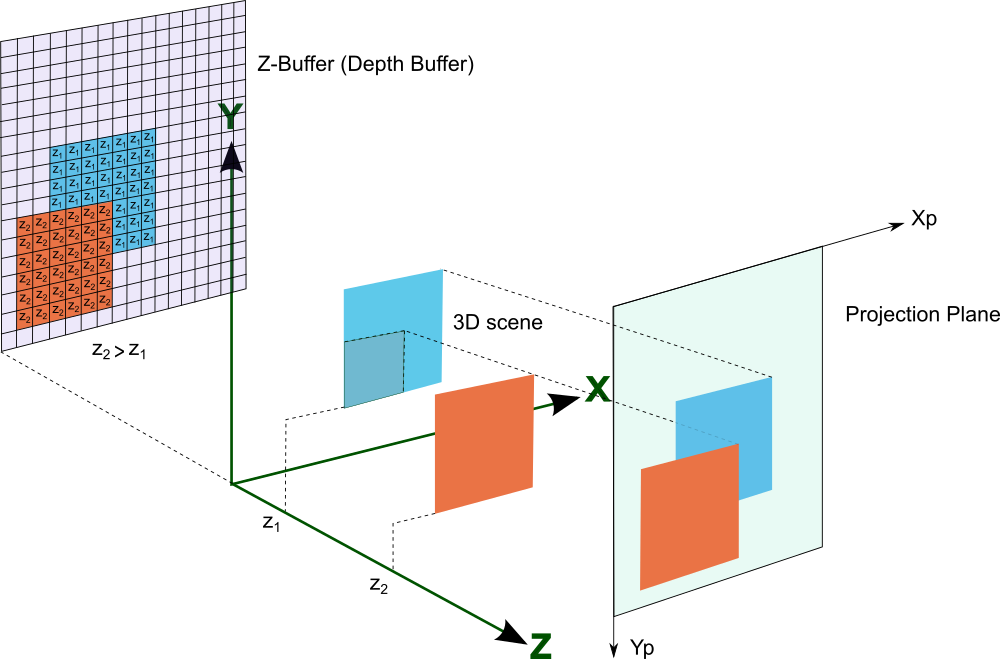
\includegraphics[scale=0.55]{zbuffer}
	\caption{Работа алгоритма z-буфер}
	\label{fig:zbuffer}
\end{figure}	

\subsubsection{Выбор алгоритма для удаления задних линий}
\hspace{0.6cm}Алгоритмы, работающие в трехмерном пространстве, и алгоритм художника не подходят из-за высокой трудозатратности, т. к. число обрабатываемых точек модели полотна флага велико. Для поставленной задачи будет использоваться алгоритм Z-буфера.

\subsection{Метод тонирования Гуро}
\hspace{0.6cm}Метод тонирования Гуро основан на интерполяции интенсивности, данный подход к закраске объекта позволяет устранить дискретность изменения интенсивности.

\vspace{0.3cm}Процесс закраски Гуро можно разделить на четыре этапа:
\begin{enumerate}
	\item вычисление нормалей ко всем полигонам;
	\item определение нормали в вершинах путем усреднения нормалей по всем полигональным граням;
	\item вычисление значений интенсивности в вершинах, используя нормали в вершинах и применяя произвольный метод закраски;
	\item закрашивание многоугольника путем линейной интерполяции значений интенсивности в вершинах (сначала вдоль каждого ребра, а затем между ребрами).
\end{enumerate}


\begin{figure}[ht!]
	\centering
	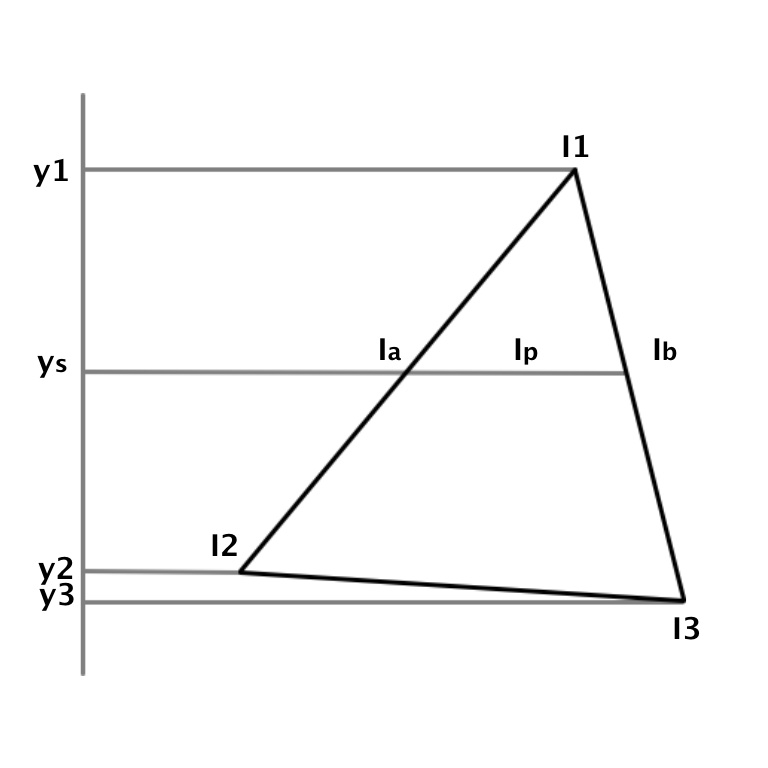
\includegraphics[scale=0.45]{guro}
	\caption{Интерполяция интенсивностей}
	\label{fig:guro}
\end{figure}

\newpage

\vspace{0.3cm}Интерполяция интенсивностей работает следующим образом: для всех ребер запоминается начальная интенсивность, изменение интенсивности при каждом шаге по координате y. Затем, заполнение видимого интервала производится путем интерполяции между значениями интенсивности на ребрах, ограничивающих интервал (рис. \ref{fig:guro}).

\vspace{0.3cm}Ниже приведены три формулы вычисления интенсивности цвета для каждой границы строки от $I_a$ до $I_b$, приведенной на рис. \ref{fig:guro}.

\begin{equation}
I_a = I_1\frac{y_s-y_2}{y_1-y_2} + I_2\frac{y_1-y_s}{y_1-y_2}
\end{equation}

\begin{equation}
I_b = I_1\frac{y_s-y_3}{y_1-y_3} + I_3\frac{y_1-y_s}{y_1-y_3}
\end{equation}

\begin{equation}
I_p = I_a\frac{x_b-x_p}{x_b-x_a} + I_b\frac{x_p-x_a}{x_b-x_a}
\end{equation}

\section{Метод ключевых кадров}
\hspace{0.6cm}Метод ключевых кадров является базовой анимацией во многих прикладных программах, и для многих программистов, незнакомых с анимированием объектов данный метод является интуитивно понятным. Основная идея использования ключевых кадров заключается в создании ключей анимации для начального и конечного положения объекта, при этом состояние объектов в промежуточных стадиях просчитывает компьютер.

\vspace{0.3cm}Термины, использующиеся в данном методе:
\begin{itemize}
	\item ключевой кадр - кадр с ключем анимации;
	\item ключ - маркер со значениями анимируемых объектов в данный момент;
	\item автоключ - процедура для отслеживания изменения параметров анимируемго объекта, может автоматически создавать ключевой кадр.
\end{itemize}

Наглядный пример работы метода ключевых кадров можно увидеть на рис. \ref{fig:keyframe}\cite{web:keyframe}.

\begin{figure}[ht!]
	\centering
	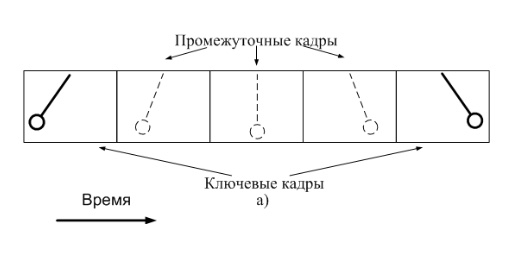
\includegraphics[scale=0.7]{keyframe}
	\caption{Работа метода ключевых кадров на примере маятника}
	\label{fig:keyframe}
\end{figure}

\vspace{0.3cm}Недостатками данного метода являются
\begin{itemize}
	\item большая трудоемкость создания и вычисления;
	\item большой объем памяти, необходимый для хранения промежуточных состояний объекта.
\end{itemize}

\section{Вывод}
\hspace{0.6cm}В данном разделе были рассмотрены алгоритм рисования линий Брезенхема, алгоритмы удаления невидимых линий художника, Z-буфера и A-буфера, метод тонировки Гуро и метод ключевых кадров. В результате сравнения в качестве алгоритма удаления невидимых линий для решения поставленной задачи был выбран алгоритм Z-буфера.
Для решении задачи изменения положения точек используется система уравнений \ref{eq:sys}, с помощью которой можно формализовать алгоритм решения.
	
